\documentclass[12pt,a4paper,titlepage]{article}
\usepackage{lab_style}
\usepackage{pdfpages}
\usepackage{eso-pic}
\usepackage{graphicx}
\usepackage{float}
\newcommand\tab[1][1cm]{\hspace*{#1}}

\graphicspath{ {./} }
  
\begin{document}

\begin{titlepage}
\selectlanguage{english}

%----------------------------------------------------------------------------------------
% TITLE PAGE INFORMATION
%----------------------------------------------------------------------------------------
  \begin{center} % Center everything on the page

  %----------------------------------------------------------------------------------------
  % HEADING SECTIONS
  %----------------------------------------------------------------------------------------
  \textsc{\large Faculty of Computers, Informatics and Microelectronics}\\[0.5cm]
  \textsc{\large Technical University of Moldova}\\[1.2cm] % Name of your university/college
  \vspace{25 mm}

  \textsc{\Large Object-Oriented Modeling and Analysis}\\[0.5cm] % Major heading such as course name
  \textsc{\large Laboratory work \#5}\\[0.5cm] % Minor heading such as course title

\newcommand{\HRule}{\rule{\linewidth}{0.5mm}} % Defines a new command for the horizontal lines, change thickness here

  %----------------------------------------------------------------------------------------
  % TITLE SECTION
  %----------------------------------------------------------------------------------------
  \vspace{10 mm}
  \HRule \\[0.4cm]
  { \LARGE \bfseries Modeling your project with Class Diagrams. SWOT Analysis. Design Principles. }\\[0.4cm] % Title of your document
  \HRule \\[1.5cm]

  %----------------------------------------------------------------------------------------
  % AUTHOR SECTION
  %----------------------------------------------------------------------------------------
      \vspace{30mm}

      \begin{minipage}{0.4\textwidth}
      \begin{flushleft} \large
      \emph{Author:}\\
      Cernei \textsc{Liviu}
      \end{flushleft}
      \end{minipage}
      ~
      \begin{minipage}{0.4\textwidth}
      \begin{flushright} \large
      \emph{Supervisor:} \\
      Mihail \textsc{Gavrilița} % Supervisor's Name
      \end{flushright}
      \end{minipage}\\[4cm]

      \vspace{5 mm}
      % If you don't want a supervisor, uncomment the two lines below and remove the section above
      %\Large \emph{Author:}\\
      %John \textsc{Smith}\\[3cm] % Your name

      %----------------------------------------------------------------------------------------
      % DATE SECTION
      %----------------------------------------------------------------------------------------

      {\large Chișinau 2018}\\[3cm] % Date, change the \today to a set date if you want to be precise

      %----------------------------------------------------------------------------------------
      % LOGO SECTION
      %----------------------------------------------------------------------------------------

      %\includegraphics{red}\\[0.5cm] % Include a department/university logo - this will require the graphicx package

      %----------------------------------------------------------------------------------------

      \vfill % Fill the rest of the page with whitespace
      \end{center}
      
\end{titlepage}

\cleardoublepage

\newpage

\pagenumbering{arabic}
\setcounter{page}{1}
\setcounter{secnumdepth}{4}

\addtocontents{toc}{\protect\thispagestyle{empty}} % no page number on the table of contents page
\cleardoublepage


\phantomsection
\addcontentsline{toc}{section}{Introduction}
\section*{Laboratory work \#5}
\phantomsection

\section{Tasks}
\begin{itemize}
	\item
	Model your application using Class Diagrams;
	\item 
	Perform the SWOT analysis of your project.
\end{itemize}

\section{Theory}

COUPLING - An indication of the strength of interconnections between program units.
Highly coupled have program units dependent on each other. Loosely coupled are made up of units that are independent or almost independent.\par

COHESION - Measure of how well module fits together.
A component should implement a single logical function or single logical entity. All the parts should contribute to the implementation.\par
SEPARATION OF CONCERNS (SoC) is a design principle for separating a computer program into distinct sections, such that each section addresses a separate concern. A concern is a set of information that affects the code of a computer program. A concern can be as general as the details of the hardware the code is being optimized for, or as specific as the name of a class to instantiate. A program that embodies SoC well is called a modular program. Modularity, and hence separation of concerns, is achieved by encapsulating information inside a section of code that has a well-defined interface. Encapsulation is a means of information hiding. Layered designs in information systems are another embodiment of separation of concerns (e.g., presentation layer, business logic layer, data access layer, persistence layer).\par

CONCEPTUAL INTEGRITY is the principle that anywhere you look in your system, you can tell that the design is part of the same overall design. This includes low-level issues such as formatting and identifier naming, but also issues such as how modules and classes are designed, etc.\par


\clearpage

\section{Class Diagrams}
In Figure ~\ref{fig:class} is represented the class diagram for the website.
\begin{figure}[H]
	\centering
	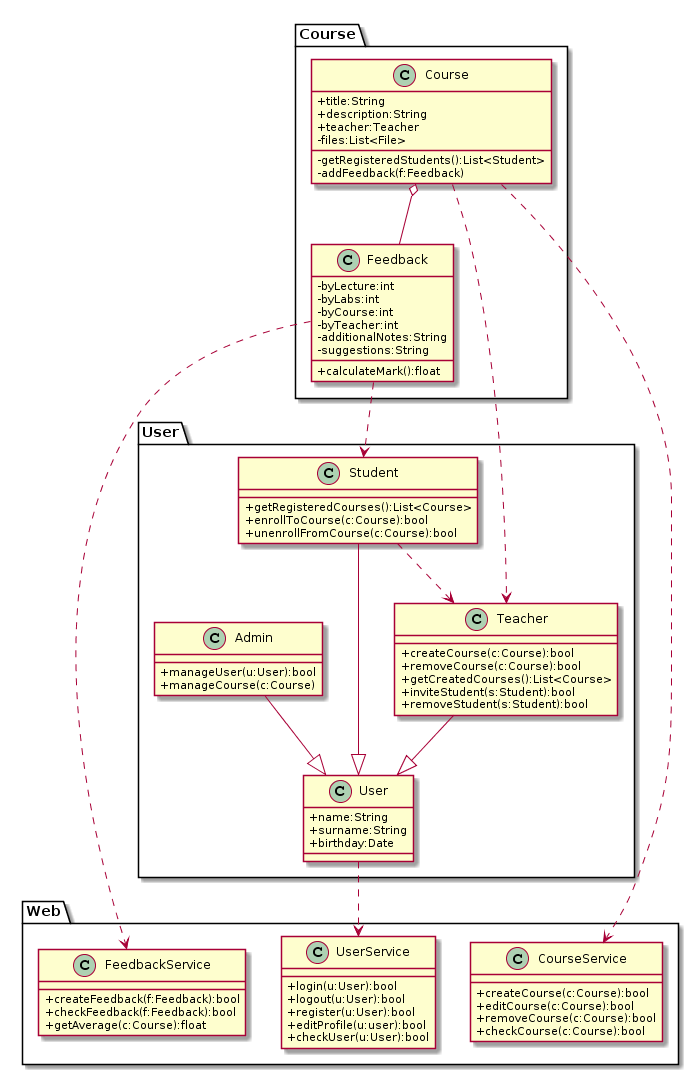
\includegraphics[width=15cm]{class}
	\caption{Class diagram}
	\label{fig:class}
\end{figure}
The diagram is divided in 3 packages: User, Web, Course. The "Course package" contains the classes Feedback and Course. Feedback is part of Course, that's why they are in agregation relationship. The "User" package contains 3 classses: Admin, Teacher and Student which inherit from the User class. The Feedback depends of Student. The Stdent depends of the Teacher (enroll/unenroll). Also the Course depends of the Teacher.\par
There is the third package, "Web". It includes FeedbackService, UserService and CourseService, each being a "dependee" for Feeback, User and Course classes respectively.

\section{SWOT analysis}
\subsection{Strengths}
\begin{itemize}
	\item Customer-centric design and messaging
	\item Useful and relevant content
	\item Intuitive navigation and search
	\item Quick and easy enrollment process
	\item Responsive design with full mobile support
\end{itemize}

\subsection{Weaknesses}
\begin{itemize}
	\item The lack of a content specialist within the web team.
	\item Minor updates and not thinking strategically.
	\item Limitations over the type of content published
\end{itemize}
\subsection{Opportunities}
\begin{itemize}
	\item New technologies to improve user experience
	\item Emerging new and untapped markets
	\item New niches and market segments
	\item New design trends to better convey messages
	\item More effective marketing tactics
	\item Positive changes in social factors
\end{itemize}
\subsection{Threats}
\begin{itemize}
	\item Competitors copying features or ideas
	\item Emergence of new competitors
	\item Changing customer needs
	\item New laws or regulations
	\item SPAM \& unsolicited advertising
	\item Upgraded browser software
\end{itemize}

\section{Conclusion}
In this laboratory work we learned to create Class Diagrams and perform SWOT analysis.

\clearpage
\cleardoublepage

\end{document}
